\documentclass[twoside]{book}

% Packages required by doxygen
\usepackage{fixltx2e}
\usepackage{calc}
\usepackage{doxygen}
\usepackage[export]{adjustbox} % also loads graphicx
\usepackage{graphicx}
\usepackage[utf8]{inputenc}
\usepackage{makeidx}
\usepackage{multicol}
\usepackage{multirow}
\PassOptionsToPackage{warn}{textcomp}
\usepackage{textcomp}
\usepackage[nointegrals]{wasysym}
\usepackage[table]{xcolor}

% NLS support packages
\usepackage[spanish]{babel}
% Font selection
\usepackage[T1]{fontenc}
\usepackage[scaled=.90]{helvet}
\usepackage{courier}
\usepackage{amssymb}
\usepackage{sectsty}
\renewcommand{\familydefault}{\sfdefault}
\allsectionsfont{%
  \fontseries{bc}\selectfont%
  \color{darkgray}%
}
\renewcommand{\DoxyLabelFont}{%
  \fontseries{bc}\selectfont%
  \color{darkgray}%
}
\newcommand{\+}{\discretionary{\mbox{\scriptsize$\hookleftarrow$}}{}{}}

% Page & text layout
\usepackage{geometry}
\geometry{%
  a4paper,%
  top=2.5cm,%
  bottom=2.5cm,%
  left=2.5cm,%
  right=2.5cm%
}
\tolerance=750
\hfuzz=15pt
\hbadness=750
\setlength{\emergencystretch}{15pt}
\setlength{\parindent}{0cm}
\setlength{\parskip}{3ex plus 2ex minus 2ex}
\makeatletter
\renewcommand{\paragraph}{%
  \@startsection{paragraph}{4}{0ex}{-1.0ex}{1.0ex}{%
    \normalfont\normalsize\bfseries\SS@parafont%
  }%
}
\renewcommand{\subparagraph}{%
  \@startsection{subparagraph}{5}{0ex}{-1.0ex}{1.0ex}{%
    \normalfont\normalsize\bfseries\SS@subparafont%
  }%
}
\makeatother

% Headers & footers
\usepackage{fancyhdr}
\pagestyle{fancyplain}
\fancyhead[LE]{\fancyplain{}{\bfseries\thepage}}
\fancyhead[CE]{\fancyplain{}{}}
\fancyhead[RE]{\fancyplain{}{\bfseries\leftmark}}
\fancyhead[LO]{\fancyplain{}{\bfseries\rightmark}}
\fancyhead[CO]{\fancyplain{}{}}
\fancyhead[RO]{\fancyplain{}{\bfseries\thepage}}
\fancyfoot[LE]{\fancyplain{}{}}
\fancyfoot[CE]{\fancyplain{}{}}
\fancyfoot[RE]{\fancyplain{}{\bfseries\scriptsize Generado por Doxygen }}
\fancyfoot[LO]{\fancyplain{}{\bfseries\scriptsize Generado por Doxygen }}
\fancyfoot[CO]{\fancyplain{}{}}
\fancyfoot[RO]{\fancyplain{}{}}
\renewcommand{\footrulewidth}{0.4pt}
\renewcommand{\chaptermark}[1]{%
  \markboth{#1}{}%
}
\renewcommand{\sectionmark}[1]{%
  \markright{\thesection\ #1}%
}

% Indices & bibliography
\usepackage{natbib}
\usepackage[titles]{tocloft}
\setcounter{tocdepth}{3}
\setcounter{secnumdepth}{5}
\makeindex

% Hyperlinks (required, but should be loaded last)
\usepackage{ifpdf}
\ifpdf
  \usepackage[pdftex,pagebackref=true]{hyperref}
\else
  \usepackage[ps2pdf,pagebackref=true]{hyperref}
\fi
\hypersetup{%
  colorlinks=true,%
  linkcolor=blue,%
  citecolor=blue,%
  unicode%
}

% Custom commands
\newcommand{\clearemptydoublepage}{%
  \newpage{\pagestyle{empty}\cleardoublepage}%
}

\usepackage{caption}
\captionsetup{labelsep=space,justification=centering,font={bf},singlelinecheck=off,skip=4pt,position=top}

%===== C O N T E N T S =====

\begin{document}

% Titlepage & ToC
\hypersetup{pageanchor=false,
             bookmarksnumbered=true,
             pdfencoding=unicode
            }
\pagenumbering{alph}
\begin{titlepage}
\vspace*{7cm}
\begin{center}%
{\Large Práctica 3 }\\
\vspace*{1cm}
{\large Generado por Doxygen 1.8.13}\\
\end{center}
\end{titlepage}
\clearemptydoublepage
\pagenumbering{roman}
\tableofcontents
\clearemptydoublepage
\pagenumbering{arabic}
\hypersetup{pageanchor=true}

%--- Begin generated contents ---
\chapter{Índice de clases}
\section{Lista de clases}
Lista de las clases, estructuras, uniones e interfaces con una breve descripción\+:\begin{DoxyCompactList}
\item\contentsline{section}{\hyperlink{classDiccionario_1_1const__iterator}{Diccionario$<$ T, U $>$\+::const\+\_\+iterator} \\*T.\+D.\+A \hyperlink{classDiccionario_1_1const__iterator}{const\+\_\+iterator} }{\pageref{classDiccionario_1_1const__iterator}}{}
\item\contentsline{section}{\hyperlink{classDiccionario}{Diccionario$<$ T, U $>$} \\*T.\+D.\+A Diccioanrio }{\pageref{classDiccionario}}{}
\end{DoxyCompactList}

\chapter{Indice de archivos}
\section{Lista de archivos}
Lista de todos los archivos documentados y con descripciones breves\+:\begin{DoxyCompactList}
\item\contentsline{section}{include/\hyperlink{cola_8h}{cola.\+h} \\*Fichero cabecera del T\+DA \hyperlink{classCola}{Cola} }{\pageref{cola_8h}}{}
\item\contentsline{section}{include/{\bfseries cola.\+hpp} }{\pageref{cola_8hpp}}{}
\item\contentsline{section}{include/{\bfseries pila\+\_\+max.\+h} }{\pageref{pila__max_8h}}{}
\item\contentsline{section}{include/\hyperlink{pila__max_8hpp}{pila\+\_\+max.\+hpp} \\*Implementación del T\+DA pila\+\_\+max }{\pageref{pila__max_8hpp}}{}
\end{DoxyCompactList}

\chapter{Documentación de las clases}
\hypertarget{classCola}{}\section{Referencia de la plantilla de la Clase Cola$<$ T $>$}
\label{classCola}\index{Cola$<$ T $>$@{Cola$<$ T $>$}}


T.\+D.\+A. \hyperlink{classCola}{Cola}.  




{\ttfamily \#include $<$cola.\+h$>$}

\subsection*{Métodos públicos}
\begin{DoxyCompactItemize}
\item 
\mbox{\Hypertarget{classCola_aea3a971c7c522618f4dc972e8b4ff153}\label{classCola_aea3a971c7c522618f4dc972e8b4ff153}} 
\hyperlink{classCola_aea3a971c7c522618f4dc972e8b4ff153}{Cola} ()
\begin{DoxyCompactList}\small\item\em Constructor por defecto. \end{DoxyCompactList}\item 
\hyperlink{classCola_a2249ab5603a92fddb8bd9bb55abeaa24}{Cola} (const \hyperlink{classCola}{Cola}$<$ T $>$ \&original)
\begin{DoxyCompactList}\small\item\em Constructor de copias. \end{DoxyCompactList}\item 
\mbox{\Hypertarget{classCola_af4d55930921c93c626006ba2e842530b}\label{classCola_af4d55930921c93c626006ba2e842530b}} 
\hyperlink{classCola_af4d55930921c93c626006ba2e842530b}{$\sim$\+Cola} ()
\begin{DoxyCompactList}\small\item\em Destructor. \end{DoxyCompactList}\item 
\hyperlink{classCola}{Cola} \& \hyperlink{classCola_a2ac480681dec95b8ffeea075507849e2}{operator=} (const \hyperlink{classCola}{Cola}$<$ T $>$ \&otra)
\begin{DoxyCompactList}\small\item\em Operador de asignaci�n. \end{DoxyCompactList}\item 
\mbox{\Hypertarget{classCola_a2c746a66289cd4f90d4e43f712b72fb6}\label{classCola_a2c746a66289cd4f90d4e43f712b72fb6}} 
bool \hyperlink{classCola_a2c746a66289cd4f90d4e43f712b72fb6}{vacia} () const
\begin{DoxyCompactList}\small\item\em Comprueba si la cola est� vac�a. \end{DoxyCompactList}\item 
\mbox{\Hypertarget{classCola_a1df4ad2b50116ef22e77ad3f77b02d29}\label{classCola_a1df4ad2b50116ef22e77ad3f77b02d29}} 
T \& \hyperlink{classCola_a1df4ad2b50116ef22e77ad3f77b02d29}{frente} ()
\begin{DoxyCompactList}\small\item\em Devuelve el elemento del frente de la cola. \end{DoxyCompactList}\item 
\mbox{\Hypertarget{classCola_abd603daab25efd7131049f98ea09c175}\label{classCola_abd603daab25efd7131049f98ea09c175}} 
const T \& \hyperlink{classCola_abd603daab25efd7131049f98ea09c175}{frente} () const
\begin{DoxyCompactList}\small\item\em Devuelve el elemento del frente de una cola constante. \end{DoxyCompactList}\item 
void \hyperlink{classCola_a4a902e5805ae74f8d80c6f3267fd14c4}{poner} (const T \&elem)
\begin{DoxyCompactList}\small\item\em A�ade un elemento al final de la cola. \end{DoxyCompactList}\item 
\mbox{\Hypertarget{classCola_a320766ddc7020424052c99e5c82a105d}\label{classCola_a320766ddc7020424052c99e5c82a105d}} 
void \hyperlink{classCola_a320766ddc7020424052c99e5c82a105d}{quitar} ()
\begin{DoxyCompactList}\small\item\em Quita el elemento del frente de la cola. \end{DoxyCompactList}\item 
\mbox{\Hypertarget{classCola_a26e5b0df5411aa23114d790f0a8c023b}\label{classCola_a26e5b0df5411aa23114d790f0a8c023b}} 
int \hyperlink{classCola_a26e5b0df5411aa23114d790f0a8c023b}{num\+\_\+elementos} () const
\begin{DoxyCompactList}\small\item\em Devuelve el n�mero de elementos de la cola. \end{DoxyCompactList}\end{DoxyCompactItemize}


\subsection{Descripción detallada}
\subsubsection*{template$<$class T$>$\newline
class Cola$<$ T $>$}

T.\+D.\+A. \hyperlink{classCola}{Cola}. 

Una instancia {\itshape c} del tipo de dato abstracto \hyperlink{classCola}{Cola} sobre un dominio {\itshape T} es una sucesi�n finita de elementos del mismo con un funcionamiento {\itshape F\+I\+FO} (First In, First Out\}). En una cola, las operaciones de inserci�n tienen lugar en uno de los extremos, denominado {\itshape final} de la cola, mientras que el borrado y consulta se lleva a cabo en el otro extremo, denominado {\itshape frente} de la cola. Una cola de longitud {\itshape n} la denotamos


\begin{DoxyItemize}
\item $<$a1,a2,a3,..,an$<$
\end{DoxyItemize}

En esta cola, tendremos acceso �nicamente al elemento del {\itshape Frente}, es decir, a {\itshape a1}. El borrado o consulta de un elemento ser� sobre {\itshape a1}, mientras que la inserci�n de un nuevo elemento se har� despu�s de {\itshape an} (final de la cola).

Si n=0 diremos que la cola est� vac�a.

El espacio requerido para el almacenamiento es O(n), donde n es el n�mero de elementos de la cola.

\begin{DoxyAuthor}{Autor}
J. Fdez-\/\+Valdivia 
\end{DoxyAuthor}
\begin{DoxyDate}{Fecha}
Octubre 2011 
\end{DoxyDate}


\subsection{Documentación del constructor y destructor}
\mbox{\Hypertarget{classCola_a2249ab5603a92fddb8bd9bb55abeaa24}\label{classCola_a2249ab5603a92fddb8bd9bb55abeaa24}} 
\index{Cola@{Cola}!Cola@{Cola}}
\index{Cola@{Cola}!Cola@{Cola}}
\subsubsection{\texorpdfstring{Cola()}{Cola()}}
{\footnotesize\ttfamily template$<$class T$>$ \\
\hyperlink{classCola}{Cola}$<$ T $>$\+::\hyperlink{classCola}{Cola} (\begin{DoxyParamCaption}\item[{const \hyperlink{classCola}{Cola}$<$ T $>$ \&}]{original }\end{DoxyParamCaption})}



Constructor de copias. 


\begin{DoxyParams}{Parámetros}
{\em original} & La cola de la que se har� la copia. \\
\hline
\end{DoxyParams}


\subsection{Documentación de las funciones miembro}
\mbox{\Hypertarget{classCola_a2ac480681dec95b8ffeea075507849e2}\label{classCola_a2ac480681dec95b8ffeea075507849e2}} 
\index{Cola@{Cola}!operator=@{operator=}}
\index{operator=@{operator=}!Cola@{Cola}}
\subsubsection{\texorpdfstring{operator=()}{operator=()}}
{\footnotesize\ttfamily template$<$class T$>$ \\
\hyperlink{classCola}{Cola}$<$ T $>$ \& \hyperlink{classCola}{Cola}$<$ T $>$\+::operator= (\begin{DoxyParamCaption}\item[{const \hyperlink{classCola}{Cola}$<$ T $>$ \&}]{otra }\end{DoxyParamCaption})}



Operador de asignaci�n. 


\begin{DoxyParams}{Parámetros}
{\em otra} & La cola que se va a asignar. \\
\hline
\end{DoxyParams}
\mbox{\Hypertarget{classCola_a4a902e5805ae74f8d80c6f3267fd14c4}\label{classCola_a4a902e5805ae74f8d80c6f3267fd14c4}} 
\index{Cola@{Cola}!poner@{poner}}
\index{poner@{poner}!Cola@{Cola}}
\subsubsection{\texorpdfstring{poner()}{poner()}}
{\footnotesize\ttfamily template$<$class T$>$ \\
void \hyperlink{classCola}{Cola}$<$ T $>$\+::poner (\begin{DoxyParamCaption}\item[{const T \&}]{elem }\end{DoxyParamCaption})}



A�ade un elemento al final de la cola. 


\begin{DoxyParams}{Parámetros}
{\em elem} & Elemento que se va a a�adir. \\
\hline
\end{DoxyParams}


La documentación para esta clase fue generada a partir de los siguientes ficheros\+:\begin{DoxyCompactItemize}
\item 
include/\hyperlink{cola_8h}{cola.\+h}\item 
include/cola.\+hpp\end{DoxyCompactItemize}

\hypertarget{classPilaMax}{}\section{Referencia de la plantilla de la Clase Pila\+Max$<$ T $>$}
\label{classPilaMax}\index{Pila\+Max$<$ T $>$@{Pila\+Max$<$ T $>$}}


T.\+D.\+A. Pila\+\_\+\+Max.  




{\ttfamily \#include $<$pila\+\_\+max.\+h$>$}

\subsection*{Métodos públicos}
\begin{DoxyCompactItemize}
\item 
\mbox{\Hypertarget{classPilaMax_a75df9c3622957f933f913b2f09d7bca3}\label{classPilaMax_a75df9c3622957f933f913b2f09d7bca3}} 
\hyperlink{classPilaMax_a75df9c3622957f933f913b2f09d7bca3}{Pila\+Max} ()
\begin{DoxyCompactList}\small\item\em Constructor por defecto. \end{DoxyCompactList}\item 
\mbox{\Hypertarget{classPilaMax_a65d381f2d58fa40b744535aa61a95646}\label{classPilaMax_a65d381f2d58fa40b744535aa61a95646}} 
\hyperlink{classPilaMax_a65d381f2d58fa40b744535aa61a95646}{Pila\+Max} (T val)
\begin{DoxyCompactList}\small\item\em Constructor con parámetros. \end{DoxyCompactList}\item 
\hyperlink{classPilaMax_abbc833df3e55f3c4b8fc02fca156ca16}{Pila\+Max} (const \hyperlink{classPilaMax}{Pila\+Max}$<$ T $>$ \&original)
\begin{DoxyCompactList}\small\item\em Constructor de copia. \end{DoxyCompactList}\item 
\mbox{\Hypertarget{classPilaMax_afbbe8f45bdb34b49047863b26bb86f60}\label{classPilaMax_afbbe8f45bdb34b49047863b26bb86f60}} 
bool \hyperlink{classPilaMax_afbbe8f45bdb34b49047863b26bb86f60}{empty} ()
\begin{DoxyCompactList}\small\item\em Comprueba si la pila está vacía. \end{DoxyCompactList}\item 
\mbox{\Hypertarget{classPilaMax_a17d84be973a9df1e1ee51e87df045348}\label{classPilaMax_a17d84be973a9df1e1ee51e87df045348}} 
int \hyperlink{classPilaMax_a17d84be973a9df1e1ee51e87df045348}{size} () const
\begin{DoxyCompactList}\small\item\em Número de elementos de la pila. \end{DoxyCompactList}\item 
Elemento \& \hyperlink{classPilaMax_a8ededbe2b2180656cdbaa0a0a437fb65}{top} ()
\begin{DoxyCompactList}\small\item\em Obtiene el tope de la pila. \end{DoxyCompactList}\item 
const Elemento \& \hyperlink{classPilaMax_a73ea1d2e5b631b551613b2b3e2d884f3}{top} () const
\begin{DoxyCompactList}\small\item\em Obtiene el tope de la pila constante. \end{DoxyCompactList}\item 
void \hyperlink{classPilaMax_a8d444d7757bf2fd488d5ed8f34a942e0}{push} (T \&nuevo)
\begin{DoxyCompactList}\small\item\em Añade un nuevo elemento al tope. \end{DoxyCompactList}\item 
\mbox{\Hypertarget{classPilaMax_ae85a974bede13446dd9e99608f848d83}\label{classPilaMax_ae85a974bede13446dd9e99608f848d83}} 
void \hyperlink{classPilaMax_ae85a974bede13446dd9e99608f848d83}{pop} ()
\begin{DoxyCompactList}\small\item\em Borra el tope de la pila. \end{DoxyCompactList}\item 
void \hyperlink{classPilaMax_a9736ed6ed710fc403dc2d5590a0032ae}{swap} (\hyperlink{classPilaMax}{Pila\+Max}$<$ T $>$ \&otro)
\begin{DoxyCompactList}\small\item\em Intercambia el contenido de esta pila y la pasada como argumento. \end{DoxyCompactList}\item 
\hyperlink{classPilaMax}{Pila\+Max} \& \hyperlink{classPilaMax_a4a2247953a5c68c37eb0f56440988e87}{operator=} (const \hyperlink{classPilaMax}{Pila\+Max}$<$ T $>$ \&original)
\begin{DoxyCompactList}\small\item\em Oprador de asignacioón. \end{DoxyCompactList}\end{DoxyCompactItemize}


\subsection{Descripción detallada}
\subsubsection*{template$<$class T$>$\newline
class Pila\+Max$<$ T $>$}

T.\+D.\+A. Pila\+\_\+\+Max. 

Una instancia {\itshape c} del tipo de dato abstracto \hyperlink{classPilaMax}{Pila\+Max} sobre un dominio {\itshape T} es una sucesión finita de elementos del mismo con un funcionamiento {\itshape L\+I\+FO} (Last In, First Out\}). En una \hyperlink{classPilaMax}{Pila\+Max}, las operaciones de inserción tienen lugar en uno de los extremos, denominado {\itshape tope} de la pila, mientras que el borrado y consulta se lleva a cabo también en ese {\itshape tope}. Además, en este caso guardaremos junto a cada elemento el valor máximo de la pila hasta ese punto, denominado máximo Una pila de longitud {\itshape n} la denotamos


\begin{DoxyItemize}
\item $<$a1\+:\mbox{[}a1,m\mbox{]},a2\+:\mbox{[}a2,m\mbox{]},a3\+:\mbox{[}a3,m\mbox{]},..,an\+:\mbox{[}an,m\mbox{]}$<$
\end{DoxyItemize}

En esta pila, tendremos acceso únicamente al elemento del {\itshape tope}, es decir, a {\itshape a1}. El borrado o consulta de un elemento será sobre {\itshape a1}, la inserción de un nuevo elemento se hará antes de {\itshape a1} (principio de la pila).

Si n=0 diremos que la pila está vacía.

El espacio requerido para el almacenamiento es O(n), donde n es el número de elementos de la cola.

\begin{DoxyAuthor}{Autor}
Francisco Ruiz Adán 
\end{DoxyAuthor}
\begin{DoxyDate}{Fecha}
18/10/2019 
\end{DoxyDate}


\subsection{Documentación del constructor y destructor}
\mbox{\Hypertarget{classPilaMax_abbc833df3e55f3c4b8fc02fca156ca16}\label{classPilaMax_abbc833df3e55f3c4b8fc02fca156ca16}} 
\index{Pila\+Max@{Pila\+Max}!Pila\+Max@{Pila\+Max}}
\index{Pila\+Max@{Pila\+Max}!Pila\+Max@{Pila\+Max}}
\subsubsection{\texorpdfstring{Pila\+Max()}{PilaMax()}}
{\footnotesize\ttfamily template$<$class T $>$ \\
\hyperlink{classPilaMax}{Pila\+Max}$<$ T $>$\+::\hyperlink{classPilaMax}{Pila\+Max} (\begin{DoxyParamCaption}\item[{const \hyperlink{classPilaMax}{Pila\+Max}$<$ T $>$ \&}]{original }\end{DoxyParamCaption})}



Constructor de copia. 


\begin{DoxyParams}{Parámetros}
{\em original} & Pila de la que se hará la copia \\
\hline
\end{DoxyParams}


\subsection{Documentación de las funciones miembro}
\mbox{\Hypertarget{classPilaMax_a4a2247953a5c68c37eb0f56440988e87}\label{classPilaMax_a4a2247953a5c68c37eb0f56440988e87}} 
\index{Pila\+Max@{Pila\+Max}!operator=@{operator=}}
\index{operator=@{operator=}!Pila\+Max@{Pila\+Max}}
\subsubsection{\texorpdfstring{operator=()}{operator=()}}
{\footnotesize\ttfamily template$<$class T $>$ \\
\hyperlink{classPilaMax}{Pila\+Max}$<$ T $>$ \& \hyperlink{classPilaMax}{Pila\+Max}$<$ T $>$\+::operator= (\begin{DoxyParamCaption}\item[{const \hyperlink{classPilaMax}{Pila\+Max}$<$ T $>$ \&}]{original }\end{DoxyParamCaption})}



Oprador de asignacioón. 


\begin{DoxyParams}{Parámetros}
{\em original} & la pila que se va asignar \\
\hline
\end{DoxyParams}
\mbox{\Hypertarget{classPilaMax_a8d444d7757bf2fd488d5ed8f34a942e0}\label{classPilaMax_a8d444d7757bf2fd488d5ed8f34a942e0}} 
\index{Pila\+Max@{Pila\+Max}!push@{push}}
\index{push@{push}!Pila\+Max@{Pila\+Max}}
\subsubsection{\texorpdfstring{push()}{push()}}
{\footnotesize\ttfamily template$<$class T $>$ \\
void \hyperlink{classPilaMax}{Pila\+Max}$<$ T $>$\+::push (\begin{DoxyParamCaption}\item[{T \&}]{nuevo }\end{DoxyParamCaption})}



Añade un nuevo elemento al tope. 


\begin{DoxyParams}{Parámetros}
{\em nuevo} & Valor a añdir en el tope \\
\hline
\end{DoxyParams}
\mbox{\Hypertarget{classPilaMax_a9736ed6ed710fc403dc2d5590a0032ae}\label{classPilaMax_a9736ed6ed710fc403dc2d5590a0032ae}} 
\index{Pila\+Max@{Pila\+Max}!swap@{swap}}
\index{swap@{swap}!Pila\+Max@{Pila\+Max}}
\subsubsection{\texorpdfstring{swap()}{swap()}}
{\footnotesize\ttfamily template$<$class T $>$ \\
void \hyperlink{classPilaMax}{Pila\+Max}$<$ T $>$\+::swap (\begin{DoxyParamCaption}\item[{\hyperlink{classPilaMax}{Pila\+Max}$<$ T $>$ \&}]{otro }\end{DoxyParamCaption})}



Intercambia el contenido de esta pila y la pasada como argumento. 


\begin{DoxyParams}{Parámetros}
{\em otro} & pila con la que intercambiar el contenido \\
\hline
\end{DoxyParams}
\begin{DoxyPostcond}{Postcondición}
Ambas pilas quedan modiciadas 
\end{DoxyPostcond}
\mbox{\Hypertarget{classPilaMax_a8ededbe2b2180656cdbaa0a0a437fb65}\label{classPilaMax_a8ededbe2b2180656cdbaa0a0a437fb65}} 
\index{Pila\+Max@{Pila\+Max}!top@{top}}
\index{top@{top}!Pila\+Max@{Pila\+Max}}
\subsubsection{\texorpdfstring{top()}{top()}\hspace{0.1cm}{\footnotesize\ttfamily [1/2]}}
{\footnotesize\ttfamily template$<$class T $>$ \\
\hyperlink{classPilaMax}{Pila\+Max}$<$ T $>$\+::Elemento \& \hyperlink{classPilaMax}{Pila\+Max}$<$ T $>$\+::top (\begin{DoxyParamCaption}{ }\end{DoxyParamCaption})}



Obtiene el tope de la pila. 

\begin{DoxyReturn}{Devuelve}
Valor del tope 
\end{DoxyReturn}
\mbox{\Hypertarget{classPilaMax_a73ea1d2e5b631b551613b2b3e2d884f3}\label{classPilaMax_a73ea1d2e5b631b551613b2b3e2d884f3}} 
\index{Pila\+Max@{Pila\+Max}!top@{top}}
\index{top@{top}!Pila\+Max@{Pila\+Max}}
\subsubsection{\texorpdfstring{top()}{top()}\hspace{0.1cm}{\footnotesize\ttfamily [2/2]}}
{\footnotesize\ttfamily template$<$class T $>$ \\
const \hyperlink{classPilaMax}{Pila\+Max}$<$ T $>$\+::Elemento \& \hyperlink{classPilaMax}{Pila\+Max}$<$ T $>$\+::top (\begin{DoxyParamCaption}{ }\end{DoxyParamCaption}) const}



Obtiene el tope de la pila constante. 

\begin{DoxyReturn}{Devuelve}
Valor del tope 
\end{DoxyReturn}


La documentación para esta clase fue generada a partir de los siguientes ficheros\+:\begin{DoxyCompactItemize}
\item 
include/pila\+\_\+max.\+h\item 
include/\hyperlink{pila__max_8hpp}{pila\+\_\+max.\+hpp}\end{DoxyCompactItemize}

\chapter{Documentación de archivos}
\hypertarget{cola_8h}{}\section{Referencia del Archivo include/cola.h}
\label{cola_8h}\index{include/cola.\+h@{include/cola.\+h}}


Fichero cabecera del T\+DA \hyperlink{classCola}{Cola}.  


{\ttfamily \#include $<$cassert$>$}\newline
{\ttfamily \#include $<$cola.\+hpp$>$}\newline
Dependencia gráfica adjunta para cola.\+h\+:\nopagebreak
\begin{figure}[H]
\begin{center}
\leavevmode
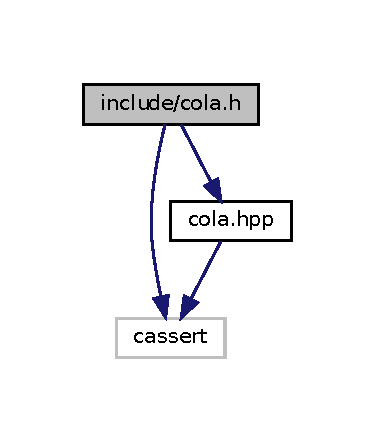
\includegraphics[width=180pt]{cola_8h__incl}
\end{center}
\end{figure}
Gráfico de los archivos que directa o indirectamente incluyen a este archivo\+:\nopagebreak
\begin{figure}[H]
\begin{center}
\leavevmode
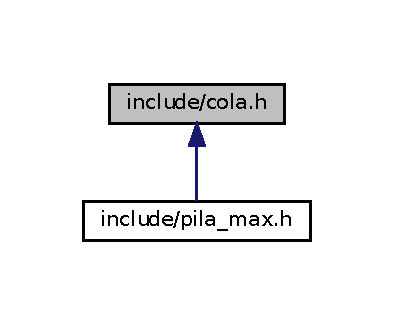
\includegraphics[width=189pt]{cola_8h__dep__incl}
\end{center}
\end{figure}
\subsection*{Clases}
\begin{DoxyCompactItemize}
\item 
class \hyperlink{classCola}{Cola$<$ T $>$}
\begin{DoxyCompactList}\small\item\em T.\+D.\+A. \hyperlink{classCola}{Cola}. \end{DoxyCompactList}\end{DoxyCompactItemize}


\subsection{Descripción detallada}
Fichero cabecera del T\+DA \hyperlink{classCola}{Cola}. 

Gestiona una secuencia de elementos con facilidades para la inserci�n y borrado de elementos en un extremo 
\hypertarget{pila__max_8hpp}{}\section{Referencia del Archivo include/pila\+\_\+max.hpp}
\label{pila__max_8hpp}\index{include/pila\+\_\+max.\+hpp@{include/pila\+\_\+max.\+hpp}}


Implementación del T\+DA pila\+\_\+max.  


Gráfico de los archivos que directa o indirectamente incluyen a este archivo\+:\nopagebreak
\begin{figure}[H]
\begin{center}
\leavevmode
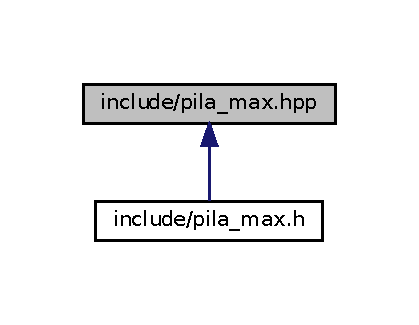
\includegraphics[width=201pt]{pila__max_8hpp__dep__incl}
\end{center}
\end{figure}


\subsection{Descripción detallada}
Implementación del T\+DA pila\+\_\+max. 


%--- End generated contents ---

% Index
\backmatter
\newpage
\phantomsection
\clearemptydoublepage
\addcontentsline{toc}{chapter}{Índice}
\printindex

\end{document}
